\documentclass{article}
\usepackage{amsmath}
\usepackage{amssymb}
\usepackage{ctex}
\usepackage[margin=2cm]{geometry} % 设置较窄的边距使文档宽一些
\usepackage{multirow} % 支持表格中的多行单元格
\usepackage{graphicx} % 用于插入图片
\title{\heiti\zihao{2} 三线摆测量物体转动惯量}
\author{\songti 王晨萱 PB23331860  孙振川  PB23081463  }
\date{2024.3.26}
\begin{document}
    \maketitle
    
\begin{abstract}
    本实验通过三线摆测量了不锈钢圆盘和不规则物体的转动惯量。
    通过对实验数据的处理和分析,我们可以计算出物体的转动惯量,
    并与理论值进行比较,从而验证实验结果的准确性。
    此外,我们还学习了如何使用三线摆进行实验,
    以及如何处理和分析实验数据。
    这些技能在物理学研究和工程应用中都是非常重要的。

    \noindent{\textbf{关键词:转动惯量;三线摆;数据处理}}
\end{abstract}


\section{引言}
    在物理学中,转动惯量是描述物体旋转特性的一个重要参数。它与物体的质量分布和旋转轴的位置有关。通过测量物体的转动惯量,可以更好地理解其运动规律和力学性质。三线摆是一种常用的实验装置,可以用于测量物体的转动惯量。通过对三线摆的实验,我们可以深入了解转动惯量的概念及其在实际应用中的重要性。
    在本实验中,我们将使用三线摆来测量物体的转动惯量。通过对实验数据的处理和分析,我们可以计算出物体的转动惯量,并与理论值进行比较,从而验证实验结果的准确性。此外,我们还将学习如何处理和分析实验数据。这些技能在物理学研究和工程应用中都是非常重要的。


\section{实验内容与设计}

\subsection{实验目的}
    \begin{enumerate}
        \item 测量物体的转动惯量
        \item 学习三线摆的使用方法
        \item 学习数据处理的方法
    \end{enumerate}

\subsection{实验仪器}
JLT-1 理论力学多功能实验台(含三线摆装置、光电检测器、尺、电子秤等);不锈钢圆盘、不规则零件(发动机摇臂)、砝码、细线。

\subsection{实验原理}
\subsubsection{转动惯量}  
转动惯量是描述刚体转动惯性大小的物理量,是刚体在转动中保持原有运动状态能力的量度。
它在旋转动力学中的角色相当于线性动力学中的质量。当刚体绕轴运动,
其合外力矩与角加速度有:$M=I \cdot \beta$ 。其中,$M$ 为刚体的合外力矩,
$\beta=\mathrm{d} \omega / \mathrm{d} t$ 为角加速度 $(\omega$ 为角速度),
$I$ 为刚体绕转动轴的转动惯量(对比 $F=m \cdot a$ )。
转动惯量在工程技术和科学研究的各个领域都有着十分广泛的应用。
例如:在设计飞轮,齿轮,涡轮等旋转机械时,需要精确计算其转动惯量,
以确保其运行的稳定性和效率;在航天器的姿态控制和轨道设计中,
转动惯量是至关重要的参数;舞蹈者在身体旋转动作中,以及运动员在跳水,
体操等项目中,都是通过调整身体姿态改变转动惯量,从而控制旋转速度。

质量连续分布的刚体,其转动惯量可写为,

$$
I=\int r^2 \mathrm{~d} m \quad\left(\text { 均质刚体可写作 } I=\rho \cdot \int r^2 \mathrm{~d} V\right)
$$

但在实际应用中,实际
的转轴并不总是通过其质心。对于相互平行的两转轴,由转动惯量的定义可以推导出平行轴定理:刚体绕任意轴的转动惯量 $I$ ,等于刚体绕通过其质心且与该轴平行的轴的转动惯量 $I_C$
,加上刚体质量 $m$ 与两轴间距离 $d$ 的平方的乘积,即

$$
I=I_c+m \cdot d^2
$$


平行轴定理提供了计算刚体绕任意平行轴转动惯量的方法。根据平行轴定理,我们只需知道刚体绕质心轴的转动惯量,即可求出绕任意平行轴的转动惯量。
    
\subsubsection{刚体转动惯量的测量}

    
    
    
    
    
用数学方法计算其转动惯量是非常困难的,因而大多采用实验方法来测定。
三线摆是一个简单的物理实验装置,用于测量物体的转动惯量。
它由一个悬挂在三根细线上的物体组成。当物体绕其中心轴旋转时,
三根细线会产生不同的张力,从而影响物体的转动惯量。通过测量这些张力和角位移,
可以计算出物体的转动惯量。
如图所示,设摆线长度为 1,圆盘质量为 $m$ ,摆线与云盘接点所在圆盘半径为 $r$ ,圆盘转角为 $\varphi$ ,摆线与垂直线的偏角为 $\alpha$ 。摆线与圆盘接点的偏摆位移可近似为:

$$
 s=r \cdot \varphi=1 \cdot \alpha \quad \text { (当偏摆至最大时) } s_{\text {max }}=r \cdot \varphi_{\text {max }}=1 \cdot \alpha_{\text {max }} 
$$      
设三线摆做初始转角为 0,角频率为 $\omega$ 的简谐振动,则有:
        
$$
\varphi=\varphi_{\max } \sin \omega t, \quad \beta_{\text {max }}=\left(\frac{\mathrm{d} \varphi}{\mathrm{~d} t}\right)_{\max }=\varphi_{\max } a
$$   
从而圆盘转动的最大动能为:
    
$$
E_{k, \max }=\frac{1}{2} I \beta_{\max }^2=\frac{1}{2} I \varphi_{\max }^2 \omega^2
$$ 
而三线摆悬挂圆盘扭转时最大势能为:

$$
E_{p, \max }=m g \cdot 1 \cdot\left(1-\cos \alpha_{\max }\right)
$$   
泰勒展开余弦函数,舍去高阶项,有
    
$$
E_{p, \max } \approx m g \cdot l \cdot \frac{\alpha_{\max }^2}{2}=\frac{1}{2} m g \frac{r^2}{l} \varphi_{\max }^2
$$
对于保守系统,$E_{k, \text { max }}=E_{p, \text { max }}$ ,由此推得:
    
$$
I=\frac{m g r^2}{l \omega^2}=\frac{m g r^2}{l(2 \pi f)^2}=\left(\frac{T}{2 \pi}\right)^2 \cdot \frac{m g r^2}{l}
$$
    
\section{实验步骤}
本实验用三线摆方法测量物体转动惯量,包括直接测量规则圆盘转动惯量和等效法测量
不规则物体转动惯量两部分内容。 
\subsection{三线摆测规则圆盘的转动惯量 }

\begin{enumerate}
    \item 打开 JLT-1 理论力学多功能实验台的电源,在实验台控制面板上以用户名 01,密码 01 登陆实验界面。
    \item 点击进入实验台屏幕界面上的"测量转动惯量实验"。测量不锈钢圆盘的质量(注意记录台秤零点)。并以游标卡尺测量圆盘的直径 $R$ 。
    \item 点击进入实验台屏幕界面上的"均质转动惯量实验"。
    \item 拧松实验台右边的转轮锁定开关,摇动手轮,将右边的一个圆盘下放。
    \item 测量有机玻璃圆盘上摆线接点所在的半径。
    \item 将不锈钢圆盘置于有机玻璃圆盘上,使两者中心重合。
    \item 调整圆盘高度至某摆线长 $L$ 处,锁紧手轮。
    \item 以水平仪检测圆盘是否水平,若不平则调至水平。
    \item 待圆盘静止,顺时针摇动底部手柄,使底部支架上行并刚好托住圆盘,旋转支架至一个微小的角度(小于 6 度),然后反向(逆时针)快速摇动底部支架手柄,使之释放圆盘,圆盘开始摆动。
    \item 在屏幕上输入摆线长度,点击“开始”按钮,等待数据显示;再次点击“开始”按钮,记录第二组数据。完成两次测量。
    \item 停止圆盘摆动,重复步骤 8 和 9,测量 3 组(每组 2 次)相同摆线长度下的周期数据。
    \item 调整摆线长度至 $L=50 \pm 2 \mathrm{~cm}, ~ 65 \pm 2 \mathrm{~cm}, ~ 80 \pm 2 \mathrm{~cm}$,重复步骤 6-10,记录 3 种不同摆线长度下的实验结果。
    \item 实验结束后,取下不锈钢圆盘并将其放回实验台抽屉中。
\end{enumerate}

\subsection{三线摆测不规则物体的转动惯量}
\begin{enumerate}
    \item 实验器材内有三物体的重量近似,分别为摇臂,钢架(悬线测重心器材)和两个圆形砝码。找出三物体,分别称重,校验三者重量情况。
    \item 测量砝码的直径,并记录。
    \item 点击进入实验台屏幕界面上的"测量转动惯量实验",并进入"非均质转动惯量实验"界面。
    \item 调整圆盘高度至某摆线长 $L$ 处,锁紧手轮。
    \item 在圆盘上分别放置摇臂和钢架,使旋转轴心(与圆盘中心对应)穿过物体重心。按实验(三)步骤 8-10 方法,分别测量两物体绕重心轴的转动惯量。每一物体分 3 组测量,每组 1~2 次,组间停止摆动后重新启动。
    \item 取下不规则物体,将两个圆柱砝码从圆盘中心孔处卡入导轨,使两砝码对称。点击进入"等质量体转动惯量实验"界面,输入质量,摆线长度,直径等。调整两砝码中心的间距,分别测量其摆动周期(两次测量取均值),并使其变换范围覆盖前面所测不规则物体的的周期。共测 5 至 8 组数据(后续采用插值方法求取不规则物体的转动惯量),请根据需要布置测点,可重复。
    \item 调整摆线长度,重复步骤 3-6,测试 2 种不同的摆线长度对结果的影响。
    \item 实验完毕,将不规则物体和砝码放回原位摆放整齐,将圆盘恢复至原来状态,并锁紧手轮。
\end{enumerate}


\section{实验数据处理}
\subsection{三线摆测规则圆盘的转动惯量}

\subsubsection{实验原始数据}

在实验中,我们测量了不锈钢圆盘的转动惯量。实验数据如下表所示:

圆盘的质量为 $m=318 \mathrm{~g}$,

圆盘的直径为 $R=99.80 \mathrm{~mm}$,

重力加速度为 $g=9.8 \mathrm{~m} / \mathrm{s}^2$。

摆线的回转半径为 $l = \frac{64.92}{\sqrt{3}} \, \mathrm{mm}$

理论计算的转动惯量为:
$$
I=\frac{1}{2} m r^2=\frac{1}{2} \cdot 0.318 \cdot \left(\frac{99.80}{2}\right)^2=39.591 \, \mathrm{\times 10^{-5}kg} \cdot \mathrm{m}^2
$$


圆盘的转动惯量 $I$ 可由下式计算:

$$
I=\left(\frac{T}{2 \pi}\right)^2 \cdot \frac{m g r^2}{L}
$$

\begin{table}[h!]
\centering
\renewcommand{\arraystretch}{1.5}
\setlength{\tabcolsep}{8pt}
\begin{tabular}{|c|c|c|c|c|c|c|c|c|c|}
\hline
\multirow{3}{*}{\textbf{No.}} & \multirow{3}{*}{\textbf{摆线长度/mm}} & \multicolumn{6}{c|}{\textbf{摆动周期/s}} & \multirow{3}{*}{\textbf{周期均值/s}} & \multirow{3}{*}{\textbf{转动惯量/ $ \mathrm{10^{-5}kg \cdot m^2} $}}  \\ \cline{3-8}
& & 1 & 2 & 3 & 4 & 5 & 6 & & \\ \hline
1 & 644 & 1.553 & 1.530 & 1.547 & 1.552 & 1.539 & 1.552 & 1.5458 & 40.082 \\ \hline
2 & 527 & 1.404 & 1.402 & 1.400 & 1.402 & 1.398 & 1.401 & 1.4012 & 40.246 \\ \hline
3 & 727 & 1.644 & 1.640 & 1.638 & 1.641 & 1.636 & 1.638 & 1.6395 & 39.941 \\ \hline
\end{tabular}
\caption{不锈钢圆盘转动测量数据}
\label{tab:raw_data}
\end{table}

误差原因,不锈钢底座的转动惯量未考虑。

摆线长度对测量值的影响:

摆线长度越长,误差越小,因为摆线长度越长,小角度近似越好,
从而使得摆动周期越长,测量值越准确。
\subsection{三线摆测不规则物体的转动惯量}
\subsubsection{不规则物体的转动惯量测量}

\begin{table}[h!]
    \centering
    \renewcommand{\arraystretch}{1.5}
    \setlength{\tabcolsep}{8pt}
    \begin{tabular}{|c|c|c|c|c|c|c|c|c|c|c|}
    \hline
    \multirow{3}{*}{\textbf{零件}} & \multirow{3}{*}{\textbf{质量 g}} & \multirow{3}{*}{\textbf{摆长/mm}} & \multicolumn{6}{c|}{\textbf{摆动周期/s}} & \multirow{3}{*}{\textbf{周期均值/s}} & \multirow{3}{*}{\textbf{转动惯量/ $ \mathrm{10^{-5}kg \cdot m^2} $}}  \\ \cline{4-9}
    & & & 1 & 2 & 3 & 4 & 5 & 6 & & \\ \hline
    1 & 644 & 727 & 1.291 & 1.281 & 1.281 &  &  &  & 1.2843 & 4.7072 \\ \hline
    1 & 644 & 464 & 1.047 & 1.049 & 1.048 &  &  &  & 1.048 & 4.8867 \\ \hline
    \end{tabular}
    \caption{不规则物体转动惯量测量数据}
    \label{tab:irregular_data}
\end{table}

\begin{figure}[h!]
    \centering
    \begin{minipage}{0.48\textwidth}
        \centering
        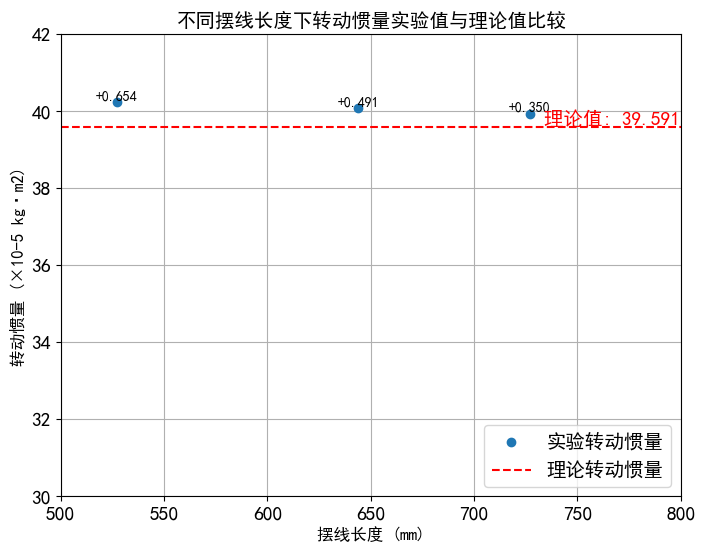
\includegraphics[width=\textwidth]{不同摆线长度下转动惯量实验值与理论值比较.png}
        \caption{不同摆线长度下转动惯量实验值与理论值比较}
        \label{fig:comparison_theory_experiment}
    \end{minipage}
    \hfill
    \begin{minipage}{0.48\textwidth}
        \centering
        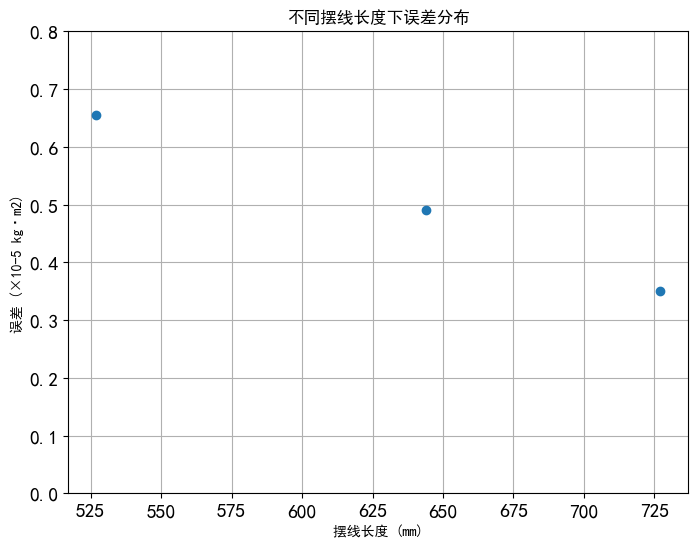
\includegraphics[width=\textwidth]{不同长度误差分布.png}
        \caption{不同长度误差分布}
        \label{fig:error_distribution}
    \end{minipage}
\end{figure}


\subsubsection{等效圆柱砝码的转动惯量测量}

根据平行轴定理,圆柱的转动惯量公式为:
$$
I = \frac{1}{8} m_s d_s^2 + m_s \left(\frac{s + d_s}{2}\right)^2
$$


其中,$m_s$ 为砝码质量,$d_s$ 为砝码直径,$s$ 为砝码间距。

实验测量数据如所示:
$m_s=79(g)$
,$d_s=18(mm)$,$g=9.8(m/s^2)$。


\begin{table}[h!]
    \centering
    \renewcommand{\arraystretch}{1.5}
    \setlength{\tabcolsep}{8pt}
    \begin{tabular}{|c|c|c|c|c|c|}
    \hline
    \multicolumn{6}{|c|}{\textbf{摆长为 727mm}} \\ \hline
    砝码间距$s$/mm & 10 & 20 & 30 & 40 & 50 \\ \hline
    摆动周期$T_1$/s & 1.014 & 1.147 & 1.302 & 1.462 & 1.648 \\ \hline
    摆动周期$T_2$/s & 1.020 & 1.122 & 1.302 & 1.658 & 1.652 \\ \hline
    平均周期$T$/s & 1.017 & 1.1345 & 1.302 & 1.660 & 1.650 \\ \hline
    \textbf{转动惯量/ $ \mathrm{10^{-5}kg \cdot m^2} $} & 1.86835 & 3.17185 & 4.87035 & 6.96385 & 9.45235 \\ \hline
    \end{tabular}
    \caption{摆长为 727mm 等效圆柱砝码的转动惯量测量数据}
    \label{tab:raw_data_simplified}
\end{table}

% 我现在需要一个表格,第一列标题为 No.,只有一行,第二列标题为摆长,只有一行,第三列标题空白,s 占一行,t 占两行,转动惯量 I 占一行,第四五六往后的列标题为 1,2,3,4,5,下面的内容为 3 行,


\begin{table}[h!]
    \centering
    \renewcommand{\arraystretch}{1.5}
    \setlength{\tabcolsep}{8pt}
    \begin{tabular}{|c|c|c|c|c|c|}
    \hline
    \multicolumn{6}{|c|}{\textbf{摆长为 464mm}} \\ \hline
    砝码间距$s$/mm & 10 & 20 & 30 & 40 & 50 \\ \hline
    摆动周期$T_1$/s & 0.819 & 0.928 & 1.056 & 1.168 & 1.318 \\ \hline
    摆动周期$T_2$/s & 0.818 & 0.924 & 1.053 & 1.172 & 1.328 \\ \hline
    平均周期$T$/s & 0.8185 & 0.926 & 1.0545 & 1.170 & 1.323 \\ \hline
    \textbf{转动惯量/ $ \mathrm{10^{-5}kg \cdot m^2} $} & 1.86835 & 3.17185 & 4.87035 & 6.96385 & 9.45235 \\ \hline
    \end{tabular}
    \caption{摆长为 464mm 等效圆柱砝码的转动惯量测量数据}
    \label{tab:raw_data_simplified}
\end{table}


\begin{figure}[h!]
    \centering
    \begin{minipage}{0.48\textwidth}
        \centering
        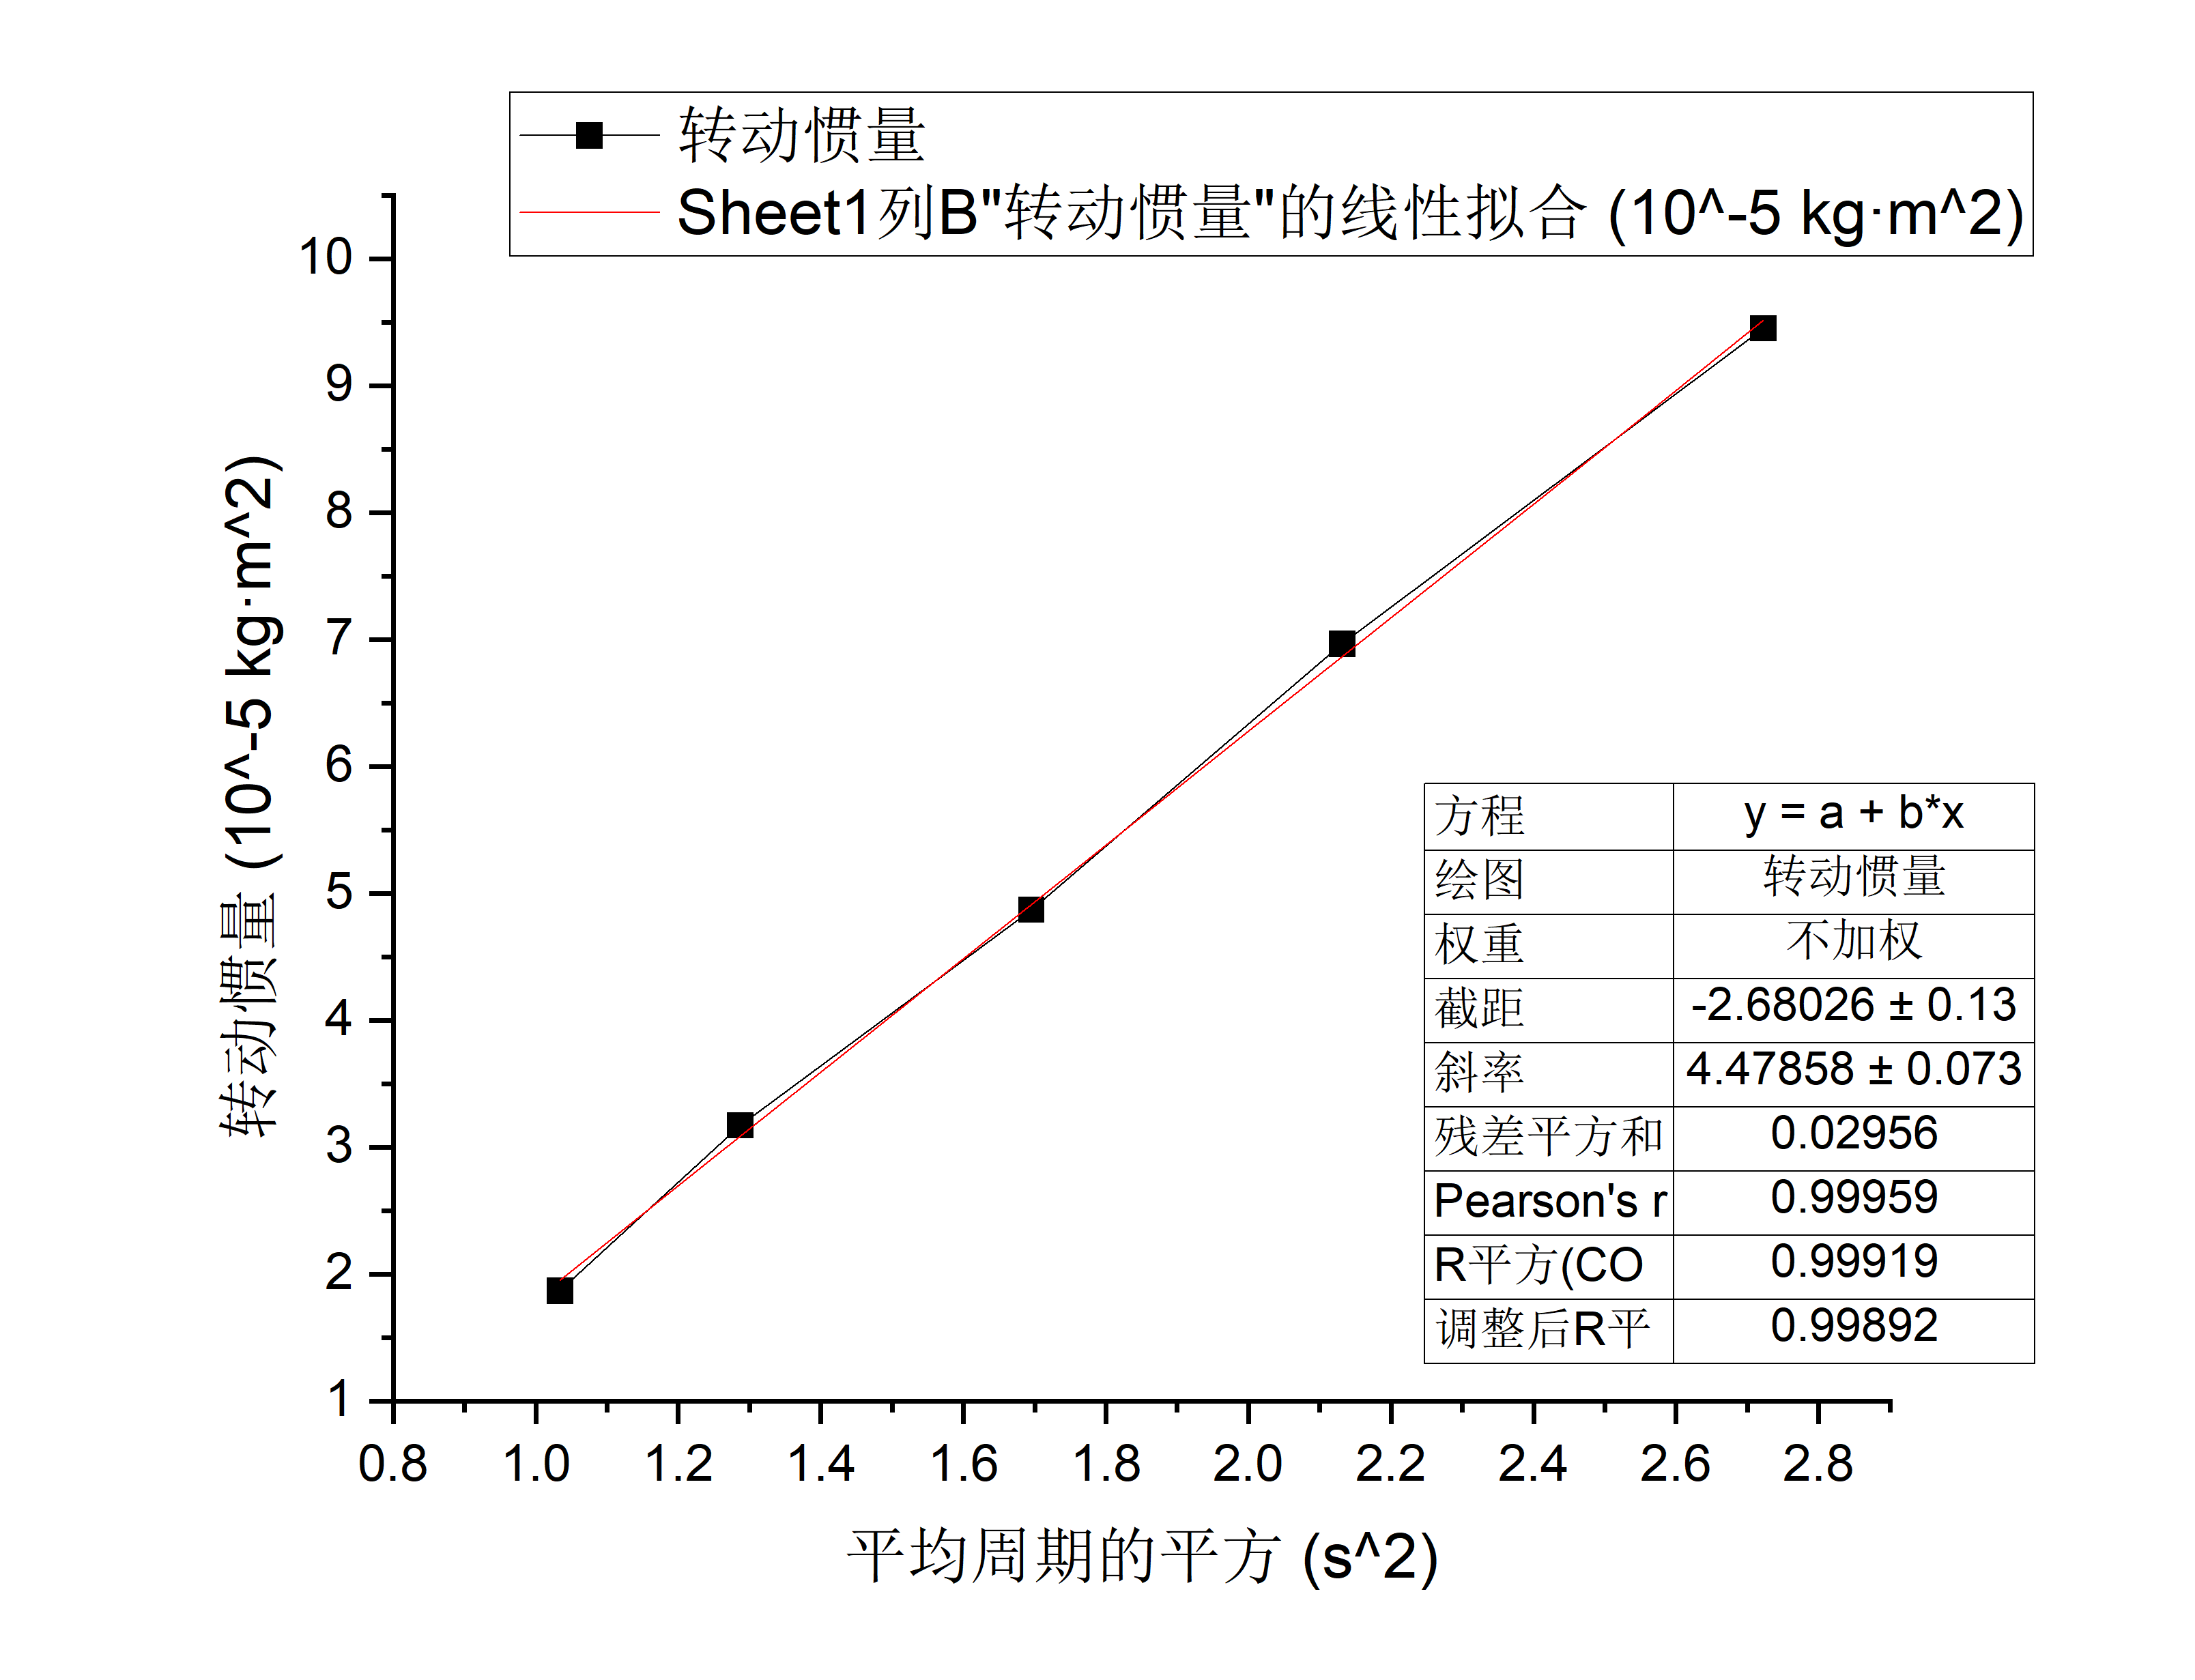
\includegraphics[width=\textwidth]{Young.png}
        \caption{摆长为 727mm 等效圆柱砝码的转动惯量测量数据}
        \label{fig:irregular_data_727}
    \end{minipage}
    \hfill
    \begin{minipage}{0.48\textwidth}
        \centering
        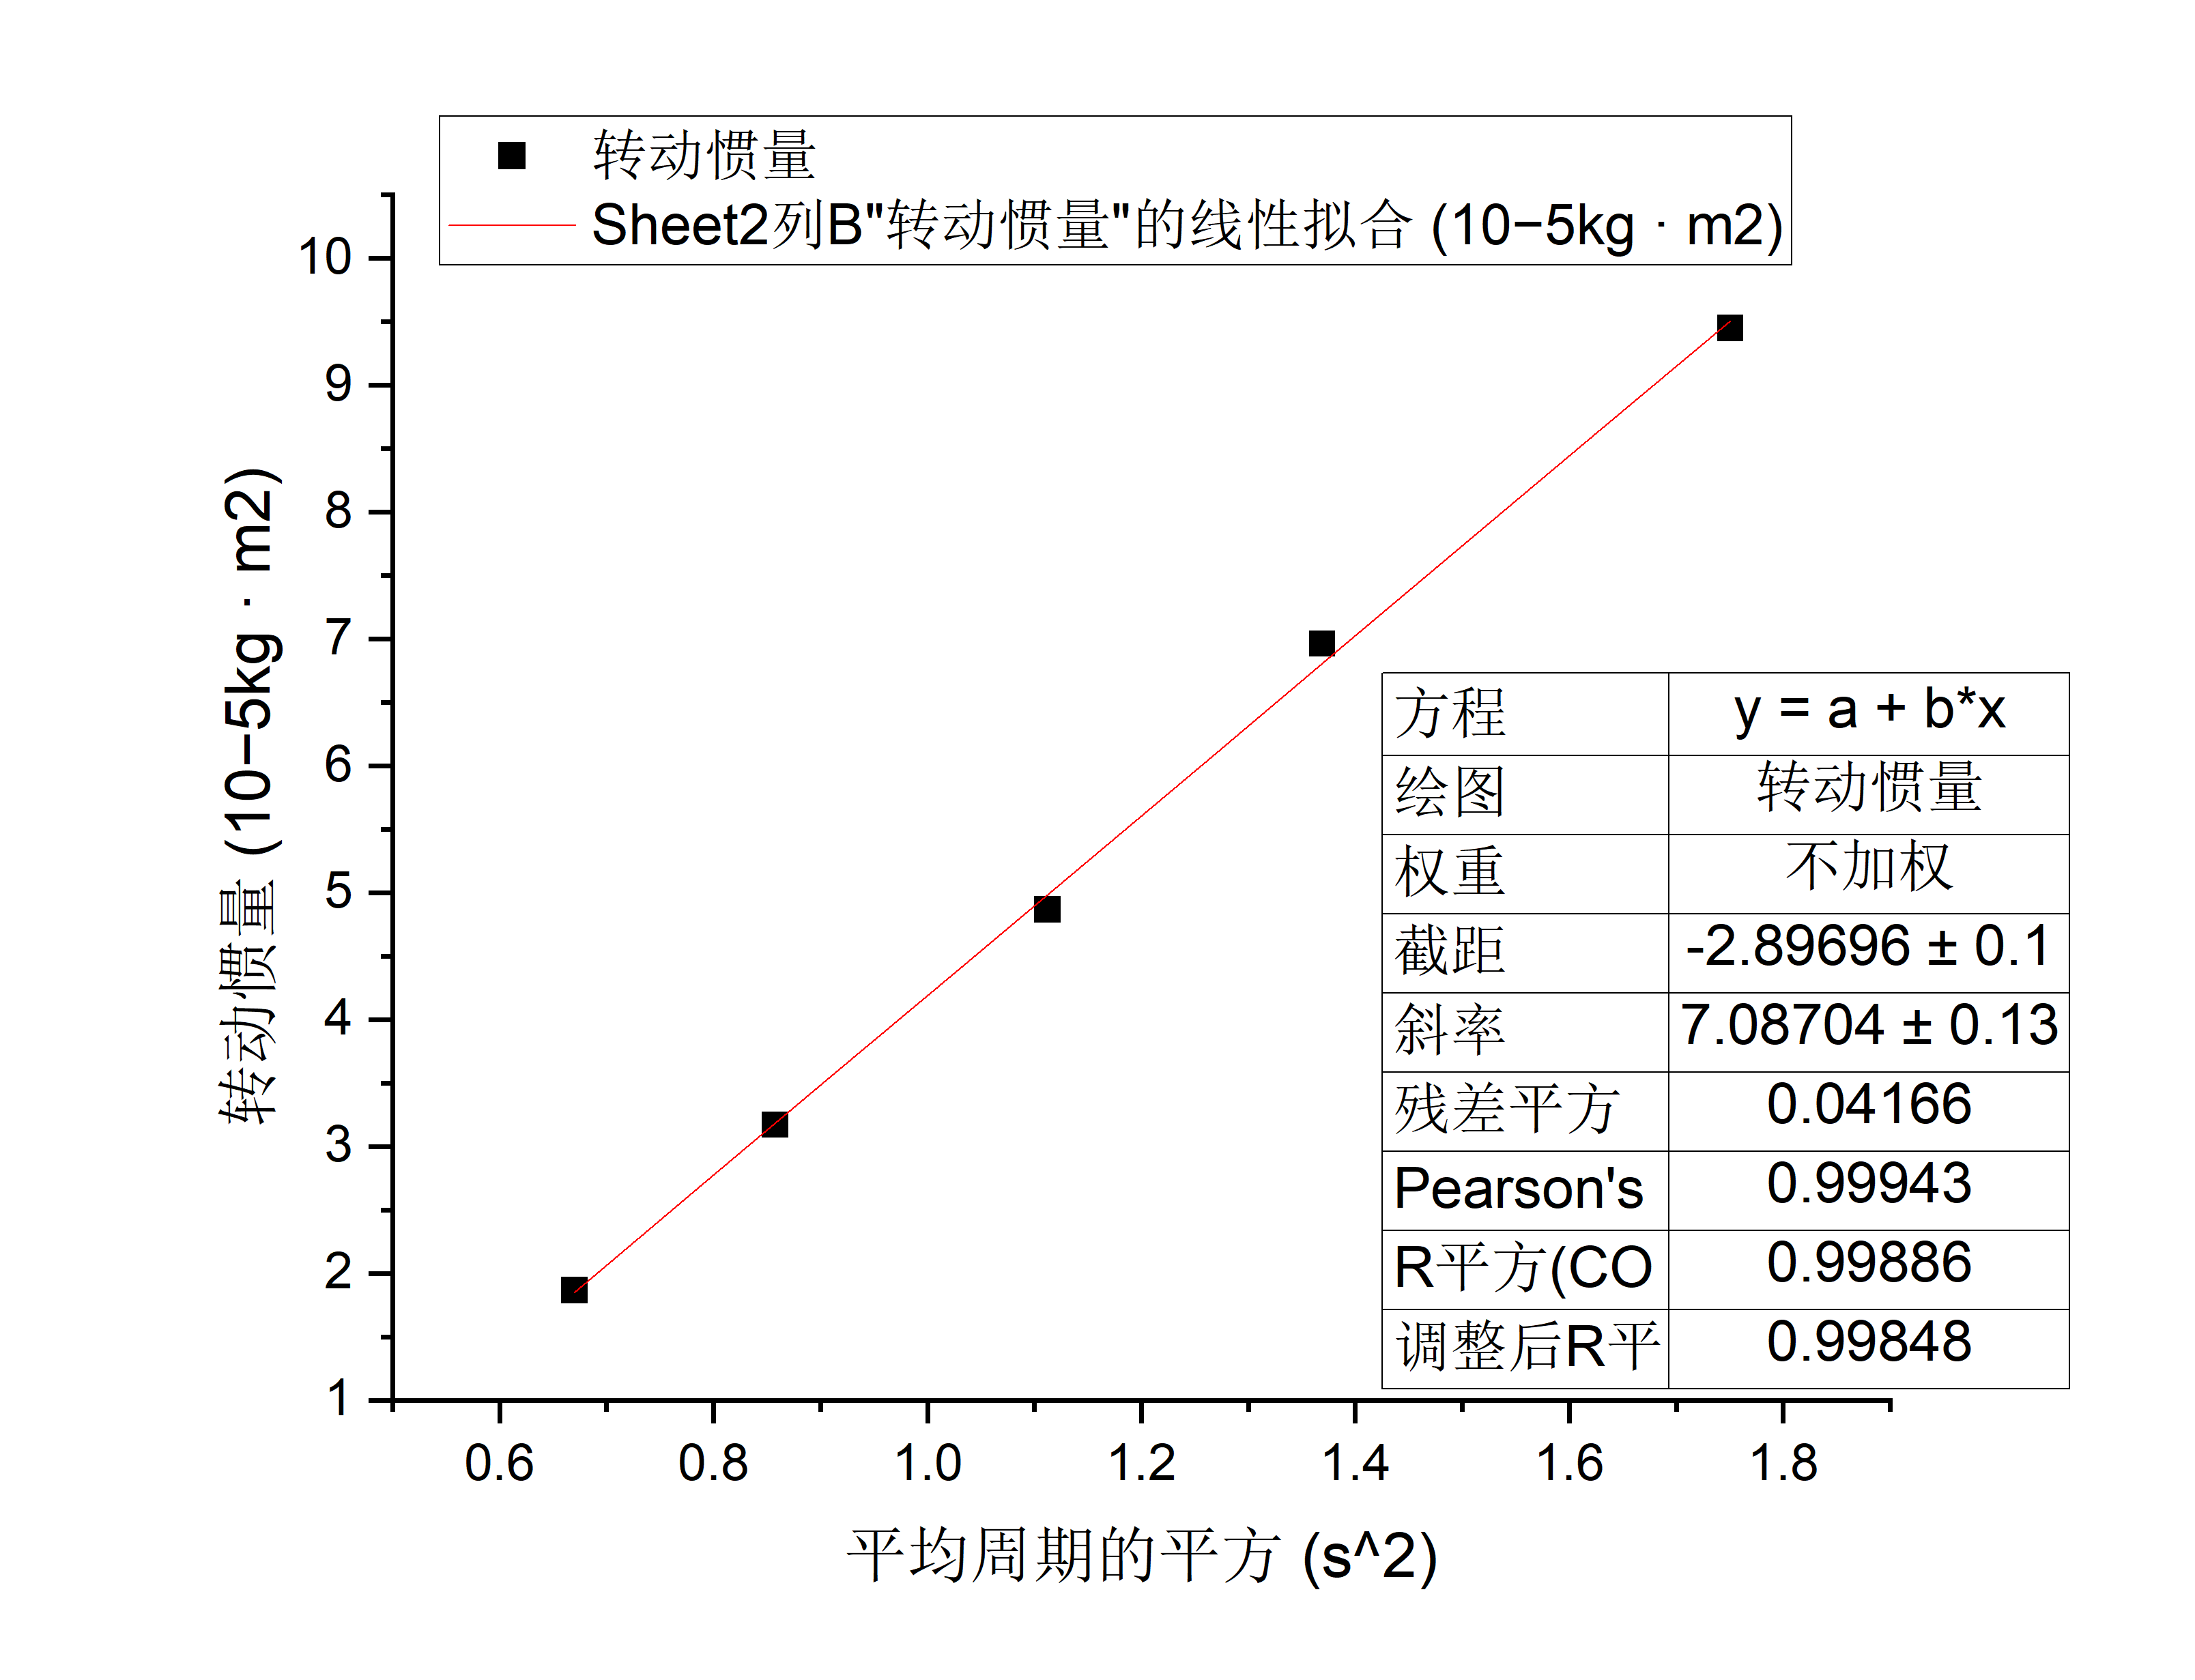
\includegraphics[width=\textwidth]{464.png}
        \caption{摆长为 464mm 等效圆柱砝码的转动惯量测量数据}
        \label{fig:irregular_data_464}
    \end{minipage}
\end{figure}

摆长为 464mm 回归方程为:
$$
I = 7.08704 \times T²  -2.8970
$$
得到
$$
I_1 = 7.08704 \times 1.048²  -2.8970=4.8867\times  \mathrm{10^{-5}kg \cdot m^2} 
$$
摆长为 727mm 回归方程为:
$$
I = 4.47858 \times T²  -2.8970
$$
得到
$$
I_2 = 4.47858 \times 1.048²  -2.68026=4.7072\times \mathrm{10^{-5}kg \cdot m^2} 
$$

\begin{figure}
    \centering
        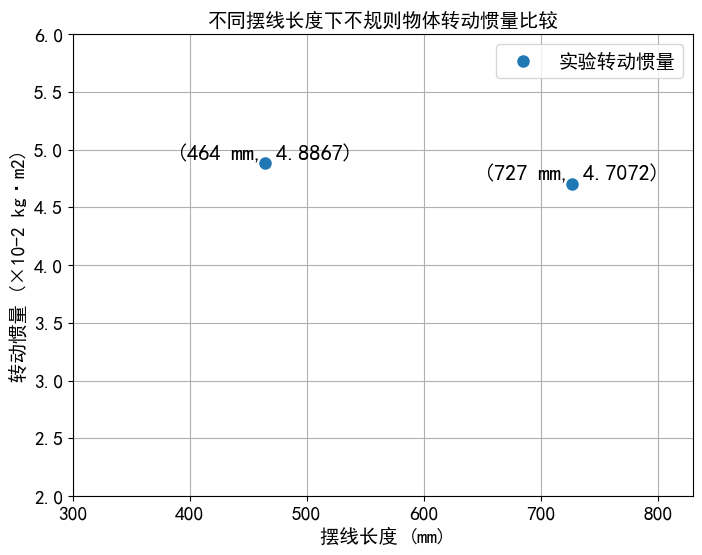
\includegraphics[width=0.5\textwidth]{不同摆线长度下不规则物体转动惯量比较.png}
        \caption{不同摆线长度下不规则物体转动惯量比较}
        \label{fig:irregular_data_464}
\end{figure}

\newpage
\section{思考题}
1.圆盘三线摆实验:

(1)如初始摆角较大,对实验结果有何影响?

由于摆角过大,三角函数的一阶近似不在成立,周期偏大,影响实验结果。

(2)设圆盘摆放时与三线接圆的圆心有 2 mm 左右的偏差,该偏差会如何影响测量的周期读数?与读数本身的重复性误差相比,这种偏差是否可以忽略?

偏差会导致转动惯量偏大,可能导致周期偏大。与读数本身的重复性误差相比,这种偏差不可以忽略。


2. 不规则物体为何不通过三线摆测得的摆动周期直接估算其转动惯量?

不规则物体的形状和质量分布较为复杂,直接利用三线摆测得的周期计算转动惯量时,往往采用的小角度近似和均质体的简化模型不再适用。这样计算出来的值容易受到局部质量分布不均、转动轴偏移等因素的影响,产生较大误差。

\section{参考文献}

[1] 理论力学实验指导书 [M] . 北京大学出版社,2007 

[2] 王惠明。应用理论力学实验 [M] . 北京高等教育出版社,2009

[3] 刘丹,侯之超。三线摆方程简化及其共振问题研究 [J]. 振动与冲击,2007,33



\end{document}